\section{Editor.\-Model.\-Project.\-Bar\-Graph Class Reference}
\label{class_editor_1_1_model_1_1_project_1_1_bar_graph}\index{Editor.\-Model.\-Project.\-Bar\-Graph@{Editor.\-Model.\-Project.\-Bar\-Graph}}


A bar graph.  




Inheritance diagram for Editor.\-Model.\-Project.\-Bar\-Graph\-:
\nopagebreak
\begin{figure}[H]
\begin{center}
\leavevmode
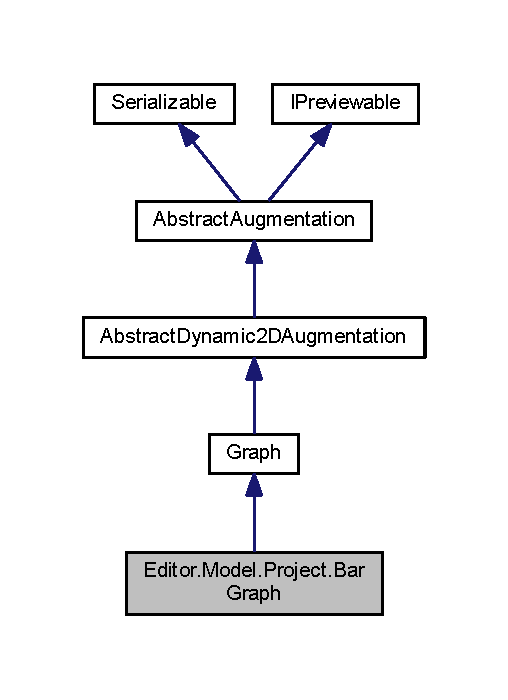
\includegraphics[width=244pt]{class_editor_1_1_model_1_1_project_1_1_bar_graph__inherit__graph}
\end{center}
\end{figure}


Collaboration diagram for Editor.\-Model.\-Project.\-Bar\-Graph\-:
\nopagebreak
\begin{figure}[H]
\begin{center}
\leavevmode
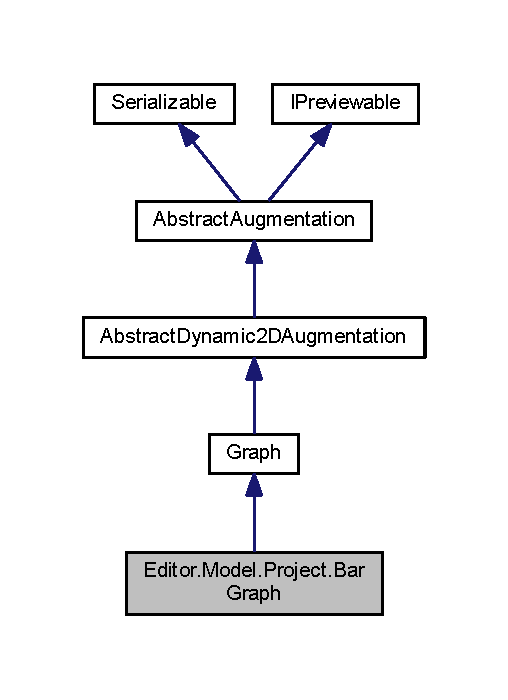
\includegraphics[width=244pt]{class_editor_1_1_model_1_1_project_1_1_bar_graph__coll__graph}
\end{center}
\end{figure}
\subsection*{Additional Inherited Members}


\subsection{Detailed Description}
A bar graph. 

Geht, 18.\-12.\-2013. 

Definition at line 20 of file Bar\-Graph.\-cs.

